\documentclass[10pt,twocolumn,letterpaper]{article}

\usepackage{cvpr}
\usepackage{times}
\usepackage{epsfig}
\usepackage{graphicx}
\usepackage{amsmath}
\usepackage{amssymb}
\usepackage{graphicx}


% Include other packages here, before hyperref.

% If you comment hyperref and then uncomment it, you should delete
% egpaper.aux before re-running latex.  (Or just hit 'q' on the first latex
% run, let it finish, and you should be clear).
\usepackage[breaklinks=true,bookmarks=false]{hyperref}

\cvprfinalcopy % *** Uncomment this line for the final submission

\def\cvprPaperID{****} % *** Enter the CVPR Paper ID here
\def\httilde{\mbox{\tt\raisebox{-.5ex}{\symbol{126}}}}

% Pages are numbered in submission mode, and unnumbered in camera-ready
%\ifcvprfinal\pagestyle{empty}\fi
\setcounter{page}{1}
\begin{document}

%%%%%%%%% TITLE
\title{Solving the Rubik's Cube without Human Interaction}

\author{Victoria Som de Cerff\\
{\tt\small vs2606@columbia.edu}
% For a paper whose authors are all at the same institution,
% omit the following lines up until the closing ``}''.
% Additional authors and addresses can be added with ``\and'',
% just like the second author.
% To save space, use either the email address or home page, not both
\and
Michael Kovalski\\
{\tt\small mhk2160@columbia.edu}
}

\maketitle
%\thispagestyle{empty}

%%%%%%%%% ABSTRACT
\begin{abstract}
We intend to investigate known methods of solving a Rubik's Cube without the need for human-tuned heuristics and reproduce similar results. 
\end{abstract}

%%%%%%%%% BODY TEXT
\section{Introduction}

A generally intelligent agent must be able to teach itself how to solve problems in complex domains with minimal human supervision.  Developing heuristics has proven to limit the search space for these problems and find good solutions, but may sometimes be too complex to come up with and may not necessarily yield optimal performance. An agent without human interaction would be able to learn promising moves by exploring the search space on it’s own and determine what states are the most optimal to be in. In the work done in “Solving the Rubik’s Cube Without Human Knowledge” they propose a method to solve a self play game without defined heuristics as rewards for intermediate states leading up to the ultimate goal state.  

Their algorithm is able to solve 100\% of randomly scrambled cubes with a scramble distance of 15, while achieving a median solve length of 30 moves.  For the first milestone the goal would be to solve a Rubik’s cube using a non-heuristic based algorithm efficiently.  I.e. not having to search the entire state space of $4.3 x 10^{19}$ possible configurations.  The second milestone would be to achieve a success rate as close as possible to that achieved in the reference paper given GPU resource constraints. 


%-------------------------------------------------------------------------

%------------------------------------------------------------------------
\section{Related Works and References}

There are previous rule based methods used to solve rubik’s cubes in a number of steps, such as knowing which layers to rotate first and how to rearrange given certain states [1]. However, this requires human intuition up front.  The upper bound was proven on how many steps it takes to solve a rubik’s cube from any starting configuration [2], although there is no simple rule based method to solve this problem. There have been previous attempts to solve this problem computationally. Heuristic based methods have been successful by using a variation of A* [3] which finds the median optimal steps away to be 18 moves. Recently, a DNN was used with featuring engineering to find the optimal route to the solution [4] but these methods take some time to run. Additionally, genetic programming has been used but fail to make optimal decisions when more than 5 steps away from the optimal solution [5]. Recent work has been done to figure out how to solve a rubik’s cube without human interaction by using the Autodidactic Iteration algorithm [6], which is similar to the AlphaZero algorithm [7] which uses Monte Carlo Tree Search to help find solutions. This algorithm can solve the rubik’s cube with 100\% success when moved 15 states away from the solved state, while on average being able to solve these puzzles in 30 steps. However, there is currently no source code for how to implement this solver. In addition, the paper uses 3 GPUs to search through the space and run neural networks for function approximation.

%-------------------------------------------------------------------------

%------------------------------------------------------------------------
\section{Problem Formulation}

Initially, we wanted to exactly replicate the work done in “Solving the Rubik’s Cube Without Human Knowledge”. In this paper, the goal is to solve the rubik's cube without the use of explicit human tuned heuristics by exploring the search space and letting a neural network be used as a guide to help through the Monte Carlo tree search, similar to the methods used in AlphaZero (insert david silver stuff here). As of now, there is no source code available for the paper. Because of this, a code base needed to be developed to help iterate through the neural network training and Monte Carlo tree search. Code was developed in python and tensorflow, where a rubik's cube simulator was built to represent the cube in a low dimensional feature space. The neural network was build to replicate the model used in the original paper, where both the value and policy are outputs. This is a more efficient way to train the network opposed to having both a value and a policy network (insert David Silver go training paper in nature here).

\subsection{Model Representation}
There are several ways to represent a rubiks cube.  Most simply, a 3x3x3 matrix.  However, since with a rubiks cube we are only concerned with the external faces, that leaves many null extraneous values internal to the matrix.   For that reason we use an alternative approach for laying out the state of our rubiks cube as 20x24 matrix where each value in the matrix has a specific meaning to the current state of the cube. 

Consider a solved cube in a fixed orientation.  There are 20 actual positions, 8 corners and 12 edge pieces.  We denote each position by the colors in that position in the fixed solved state.  For each of the 20 positions there are 24 unique color orientations that can be placed in that position.  Our state matrix is a one hot encoding of which color orientation exists each position. 

It is important for the naming convention that we afix primary (top:white / bottom: yellow), secondary (left:blue / right:green) and tertiary front:orange / back:red) planes.  

The 12 edge pieces are WB, WG, WO, WR, YB, YG, YO, YR, GO, GR, BO, BR.  In each of those unique positions, every one of those initial color orderings and their inverse can occur in that position.  i.e. the WB position can have WB, BW, WG, GW, WO, OW, etc.  Hence 24 states for the edges.  

The 8 corner pieces are WOB, WBR, WGO, WRG, YBO, YBR, YRG, YOG.  These positions are uniquely named starting in the dominant plane and reading off the remaining corner colors in a clockwise ordering.  Each color ordering can have three states by performing a clockwise rotation of the corner.  i.e. WOB-> OWB-> BOW.  Each corner position can have all 3 state for each of the 8 of the initial color orderings.  Hence 24 states for the corners. 

Now every entry in the matrix has meaningful information.  cube[position][orientation]=1 if that orientation of colors exists in that position.  Again this is a one hot encoding so only one color orientation can appear in a position at a time. 

When a face is turned the edges and corners not only move positions but will change orientation accordingly.  

The simulator maintains the state of the cube using this 20x24 representation and performs the necessary changes when given face to turn.  We have 12 valid moves.  Each of the six faces can either move clockwise or counter clockwise 90 degrees. 


\section{Methods}
As noted above, the goal was to replicate the original paper. To do this, a code base was built using the following structure. We replicated the paper exactly to initially start with a solid foundation on how the problem was solved.

\subsection{Autodidactic Iteration}
The goal of autodidactic iteration is to help efficiently observe states close to the solved rubik's cube to help guide searching in the Monte Carlo tree search by the use of a neural network. We start from a solved state rubik's cube, propogate through $N$ different cubes and determine a value for the cube's children based on the true reward and a value approximation using a neural network $f_\theta$.  The parent cube then trains this same $f_\theta$ on the optimal policy and value based on the values of the children. 
\\

Formally, the rubik's cube starts from initial solved state $S_0$. The rubik's cube is then moved from the previous state to a new state, which is done $N$ times. From each state $S_n$, $n \in N$, the rubik's cube is then expanded $\forall$ children $s_i$, where $i \ \exists \ [12]$ since there are 12 possible children. $\forall$ children, we run $f_\theta$ on the states $s_i$ to receive a value and policy. The true reward is then added to each of the value approximations made by $f_\theta$. 
The maximum value of $s_i$ is then chosen, and the $argmax \ v_i(s_i)$ is chosen as the correct policy (the route to take), where $v_i$ is the value of the maximum child. $f_\theta$ then does a forward pass using the state $S_n$ as input, and the loss is calculate based on $v_i$ and $argmax v_i$, the child with the maximum state.

In additional, it was noted in the original paper that the value approximations were weighted so that as the rubik's cube moved further away from a solved state, the values decreased. This was also implemented in our version.

\subsection{Monte Carlo Tree Search}

After the neural network is trained, we use Monte Carlo tree search to look through the space to determine which paths to take to find a solved state, using the neural network $f_\theta$ as a guide as to what paths to take. 


Initially, we start with a random state for the cube $S$. Each node of the search tree has some values assoicated with it, such as the number of times it has chosen action $a$ from state $s$, the maximum value of action $a$ from state $s$, the virtual loss function for each action $a$, and the prior probability of action $a$ from state $s$.


The tree is traversed in the following fashion: An action $a$ is selected at each node by taking the maximum value of $A=argmax_a U_{s_{t}}(a) + Q_{s_{t}}(a) $, where the two values help to explore the tree using factors such as how many times it has been visited, the maximum value of the tree, as well as hyper parameters such as $c$, which is an exploration hyperparameter, and $v$, which discourages the search from taking the same path.

When a leaf node is reached, all children are expanded and initialized, so that $N_i = 0$, $W_i = 0$, $L_i = 0$, and $P_i = p_i(f_\theta (s_i))$. The values is  then backed up all the way to the root node, where $W_s(A_t) = max(W_s(A_t), v_i(A_t)$, $N_i += 1$, $L_s -= v$.

The simulation is completed once a solves state is reached, or a maximum number of iterations are taken.

\subsection{Architecture and Design}
We used a feed forward neural network as the architecture.  The network takes in a 20x24 matrix representing the current state of the rubik's cube.  There are then two dense layers, the result of which splits apart to the derive the two outputs: 1 dimensional scalar v, representing the reward value, and a 12 dimensional vector p, representing the probability of selecting each of the possible moves for the next state.  These outputs direct the execution of the Autodidactic Iteration and Monte Carlo Tree Search.

\begin{figure}
  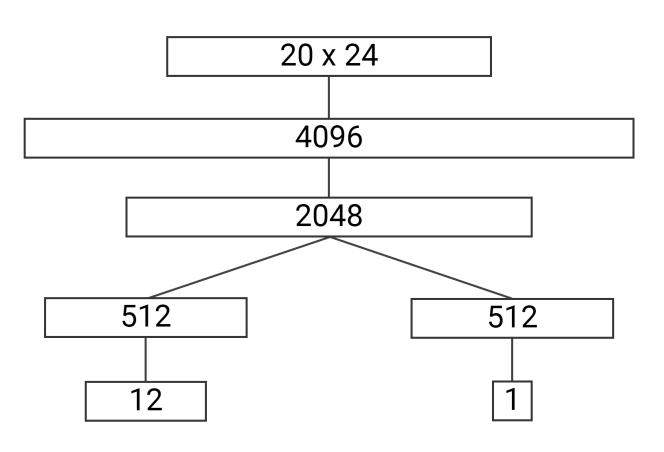
\includegraphics[width=\linewidth]{net.png}
  \caption{Neural network.}
  \label{fig:net}
\end{figure}

\subsection{Innovation}
The initial method uses a non-heuristic based approach to try and solve the rubik's cube. By doing this, human based heuristics are removed and the neural network thus approximates these heuristics for us. 

One thing that was not noted in the paper that we added into our code was ensuring that after a move, the rubik's cube did not make the opposite move afterwards to put it back to a state it had previously seen. For example, turn the top face right followed by turning the top face left would result in a configuration the rubik's cube had seen. The reason for this modification is we wanted to explore as many possible states as possible within the rubik's cube. By removing duplicate moves, we can ensure that the rubik's cube always has an unseen state during the iteration.

While the results using this method has good results in the original paper, an additional goal is to explore the hyperparameter space  and see if there are better combinations that can help to train the neural network more efficiently. Methods such as Bayesian Optimization will be used to find which hyperparamters lead to the most effective training. These hyperparameters may include layer size, number of layers, activation functions, depth of tree search in ADI, etc. The original paper notes that it uses a search depth of 1, but the code can be easily modified to search deeper into the tree when training the neural network using Autodidactic Iteration. In additional to neural network hyperparameters, the Monte Carlo tree search also has parameters that can be tweaked, such as the exploration and virtual loss, which help with exploring the tree without getting stuck always going down the same branch.

%-------------------------------------------------------------------------

%------------------------------------------------------------------------
\section{Preliminary Results}
Most of the time spent thus far was developing a code base where we can replicate the results of the original paper. A full code base was developed where a user can train the network and change a few of the hyper parameters via a command line interface. In the README.md in our github page, one can see how to easily change their training and tree search algorithms. 

Initially the model was trained for 100,000 iterations, where in each iteration, the initial state $S$ traversed 30 times. A loss function was monitored to determine how the training was doing over time. These results were a bit less than promising. In figure 1, the loss function can be seen. It seems to converge fairly quickly, but to a high value.

Why I believe this is happening is due to the additional weight parameter for the value function. In the original paper, it was noted that to keep from diverging, a weight was assigned to the value of the state, relating how far from the initial state the cube was. But, on each update of the value network, the value actually changes. By recursively assigning a weight to this new value function each time based on this weighting, it makes it very difficult for the function to converge as the value will continue to decay. One way we may handle this in the future is to use two neural networks, where one keeps track of the values unweighted and one weighted. 

One thing to note was the computational power used to train in the original paper was much more than we have available. The paper notes that using 3 GPUs they had trained for 44 hours. To do this, we had a single GPU available. The model was trained for 24 hours, but the results we had gotten were not nearly as feasible as those gotten from the paper yet. For example, using our method, we were able to solve a rubik's cube 8 steps away from the original space, but it took nearly an hour to do so. Our Monte Carlo tree search is not yet asynchronous and runs serially, so building an asynchronous tree search and longer neural networking training time may help this.

The code may need to be updated a bit more as training progresses to help speed up the process. Batch sizes were taken into consideration in training this. However, since only a single neural network is used, it makes sense to update the weights one by one, as the value of the next child depends on the previous neural network update.

%-------------------------------------------------------------------------

%------------------------------------------------------------------------


\section{Code}

While most of the methods and concepts were pulled from the paper Solving the Rubik’s Cube Without Human Knowledge (McAleer), there was not an available repository.  The model construction, neural network, and search algorithm all had to be written from scratch.  Our implementation can be found on github here: https://github.com/mkovalski/cs4995\textunderscore cube.  Our network and framework were implemented using the Tensorflow library. 

%-------------------------------------------------------------------------

%------------------------------------------------------------------------


\begin{thebibliography}{9}

\bibitem{}
https://ruwix.com/the-rubiks-cube/how-to-solve-the-rubiks-cube-beginners-method/

\bibitem{}
https://epubs.siam.org/doi/10.1137/120867366

\bibitem{}
https://www.cs.princeton.edu/courses/archive/fall06/cos402/papers/korfrubik.pdf

\bibitem{}
Robert Brunetto and Otakar Trunda. Deep heuristic-learning in the rubik’s cube domain: an experimental evaluation. 2017.

\bibitem{}
https://dl.acm.org/citation.cfm?id=2908887

\bibitem{1805.07470}
Stephen McAleer, Forest Agostinelli, Alexander Shmakov and Pierre Baldi.
\newblock Solving the Rubik's Cube Without Human Knowledge, 2018;
\newblock arXiv:1805.07470.

\bibitem{1712.01815}
David Silver, Thomas Hubert, Julian Schrittwieser, Ioannis Antonoglou, Matthew Lai, Arthur Guez, Marc Lanctot, Laurent Sifre, Dharshan Kumaran, Thore Graepel, Timothy Lillicrap, Karen Simonyan and Demis Hassabis.
\newblock Mastering Chess and Shogi by Self-Play with a General Reinforcement Learning Algorithm, 2017;
\newblock arXiv:1712.01815.

\bibitem{}
https://www.ryanheise.com/cube/cube\textunderscore laws.html


\end{thebibliography}

{\small
\bibliographystyle{ieee}
\bibliography{egbib}
}

\end{document}
